\documentclass[
	noheader
]{coursclass}

\usepackage{tikz-repère}
\usetikzlibrary{calc}

\begin{document}

\newcommand{\Definition}{
	\begin{definition}[Base orthonormée]
		\begin{minipage}{0.7\textwidth}
			Soit $O$ un point du plan, et deux vecteurs $\vec{i}$ et $\vec{j}$ dont les directions sont perpendiculaires et dont les normes sont égales à $1$.

			On dit que
			\begin{itemize}
				\item $(\vec{i},\vec{j})$ est \correctionDots{une base orthonormée} du plan ;
				\item $(O\ ;\ \vec{i},\vec{j})$ est \correctionDots{un repère orthonormé} du plan.
			\end{itemize}
		\end{minipage}
		\begin{minipage}{0.25\textwidth}
			\begin{center}
				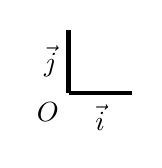
\begin{tikzpicture}[scale=0.8]
					\tikzRepere{-1.5}{1.5}{-1.5}{1.5}[][]
					\node[below left] at (0,0) {$O$};
					\draw[ultra thick,\myArrow] (0,0) -- node[below] {$\vec{i}$} ++(1,0);
					\draw[ultra thick,\myArrow] (0,0) -- node[left] {$\vec{j}$} ++(0,1);
				\end{tikzpicture}
			\end{center}
		\end{minipage}
	\end{definition}
}

\Definition

\Definition

\Definition

\Definition

\Definition

\end{document}